\subsection{CleanUNet}
We tried to replicate the training procedure stated in \cite{kong2022} for the CleanUNet model. We used 100 hours of the DNS 2020 dataset \cite{reddy2020} for training, and its corresponding test set was used for testing.

\textbf{Architecture:} The depth of the encoder or the decoder is D = 8. Each encoder/decoder layer has hidden dimension H = 64, stride S = 2, and kernel size K = 4.
The depth of the bottleneck is N = 5. Each self-attention block has 8 heads, model dimension = 512, middle dimension = 2048, no dropout, and no positional encoding.

\textbf{Optimization:} The model was trained for 50k steps with a batch size of 4. The Adam \cite{kingma2017adam} optimizer was used with a learning rate of $2\times 10^{-4}$ with a Linear Warmup Cosine Decay. The loss functions used were L1 loss and STFT loss \cite{defossez2020}.
The model was trained on 2 NVIDIA Tesla T4 GPUs. The training took 24 hours to complete. The training loss is shown in Figure \ref{fig:cleanunet-training} and metrics on the test set are shown in Table \ref{tab:cleanunet-test}.

\begin{figure}[h]
  \centering
  \begin{subfigure}{.3\textwidth}
    \centering
    % include the first image
    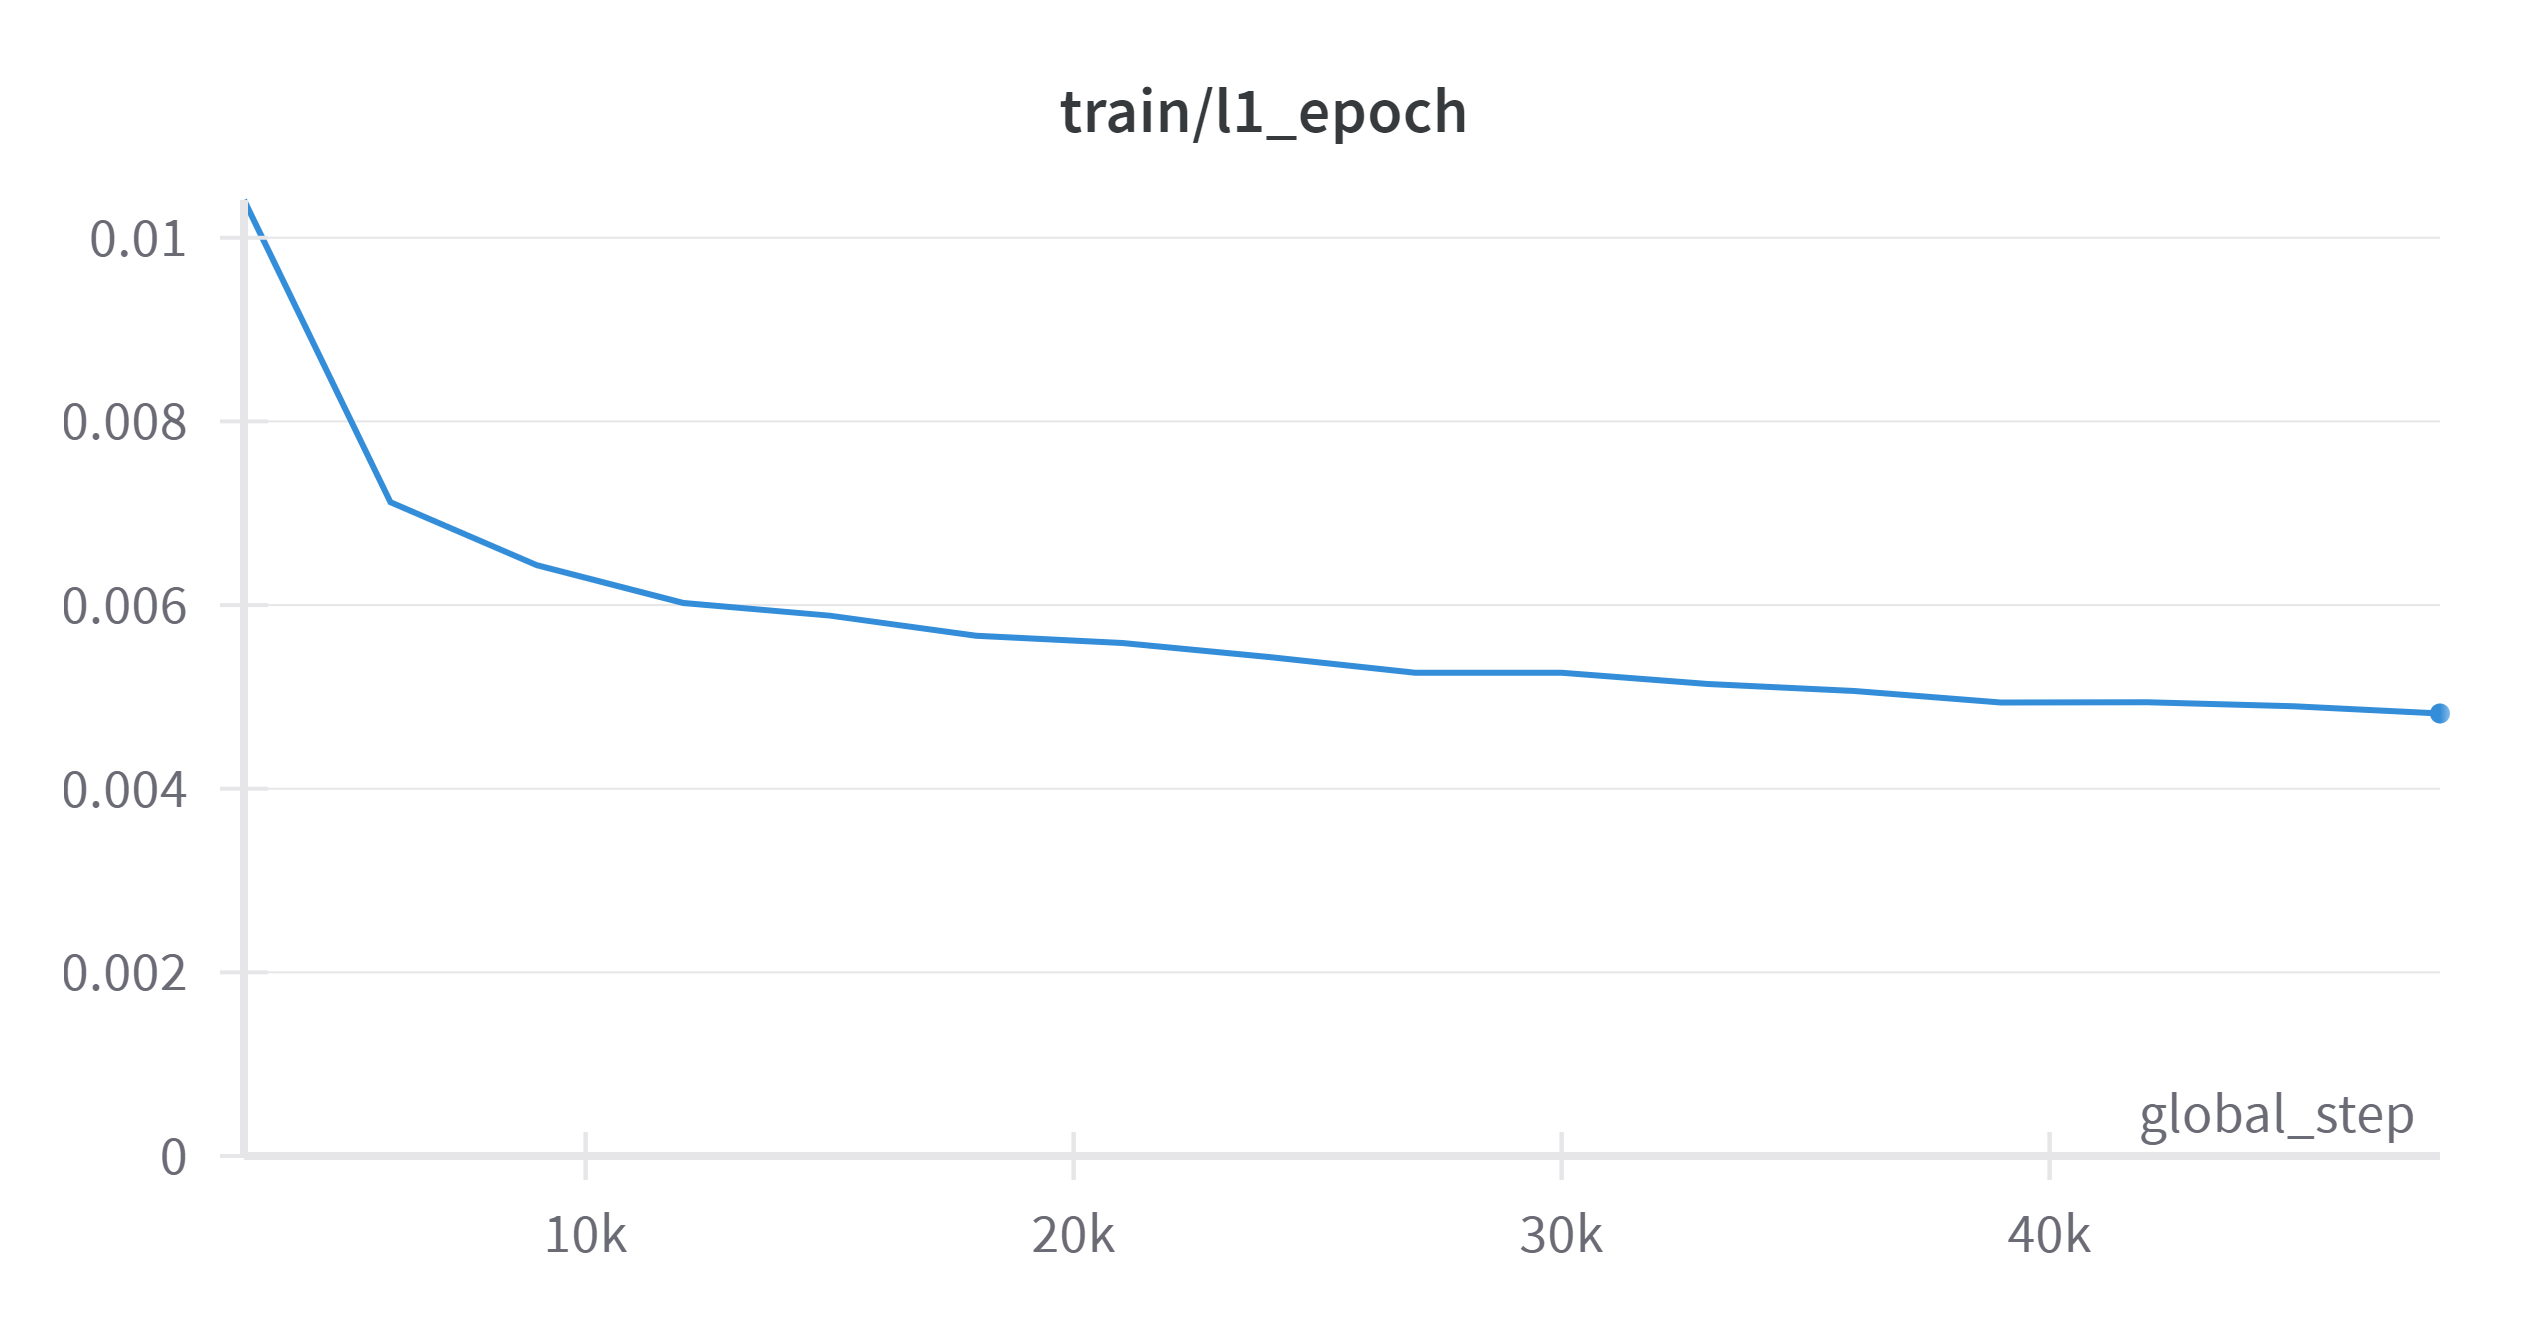
\includegraphics[width=1\linewidth]{images/experiments/cleanUnet/cleanUnet_DNS100hrs_train_l1.png}
    \caption{L1 loss reported on\\ training set.}
    \label{fig:cleanUnet_train_l1}
  \end{subfigure}
  \begin{subfigure}{.3\textwidth}
    \centering
    % includes second image
    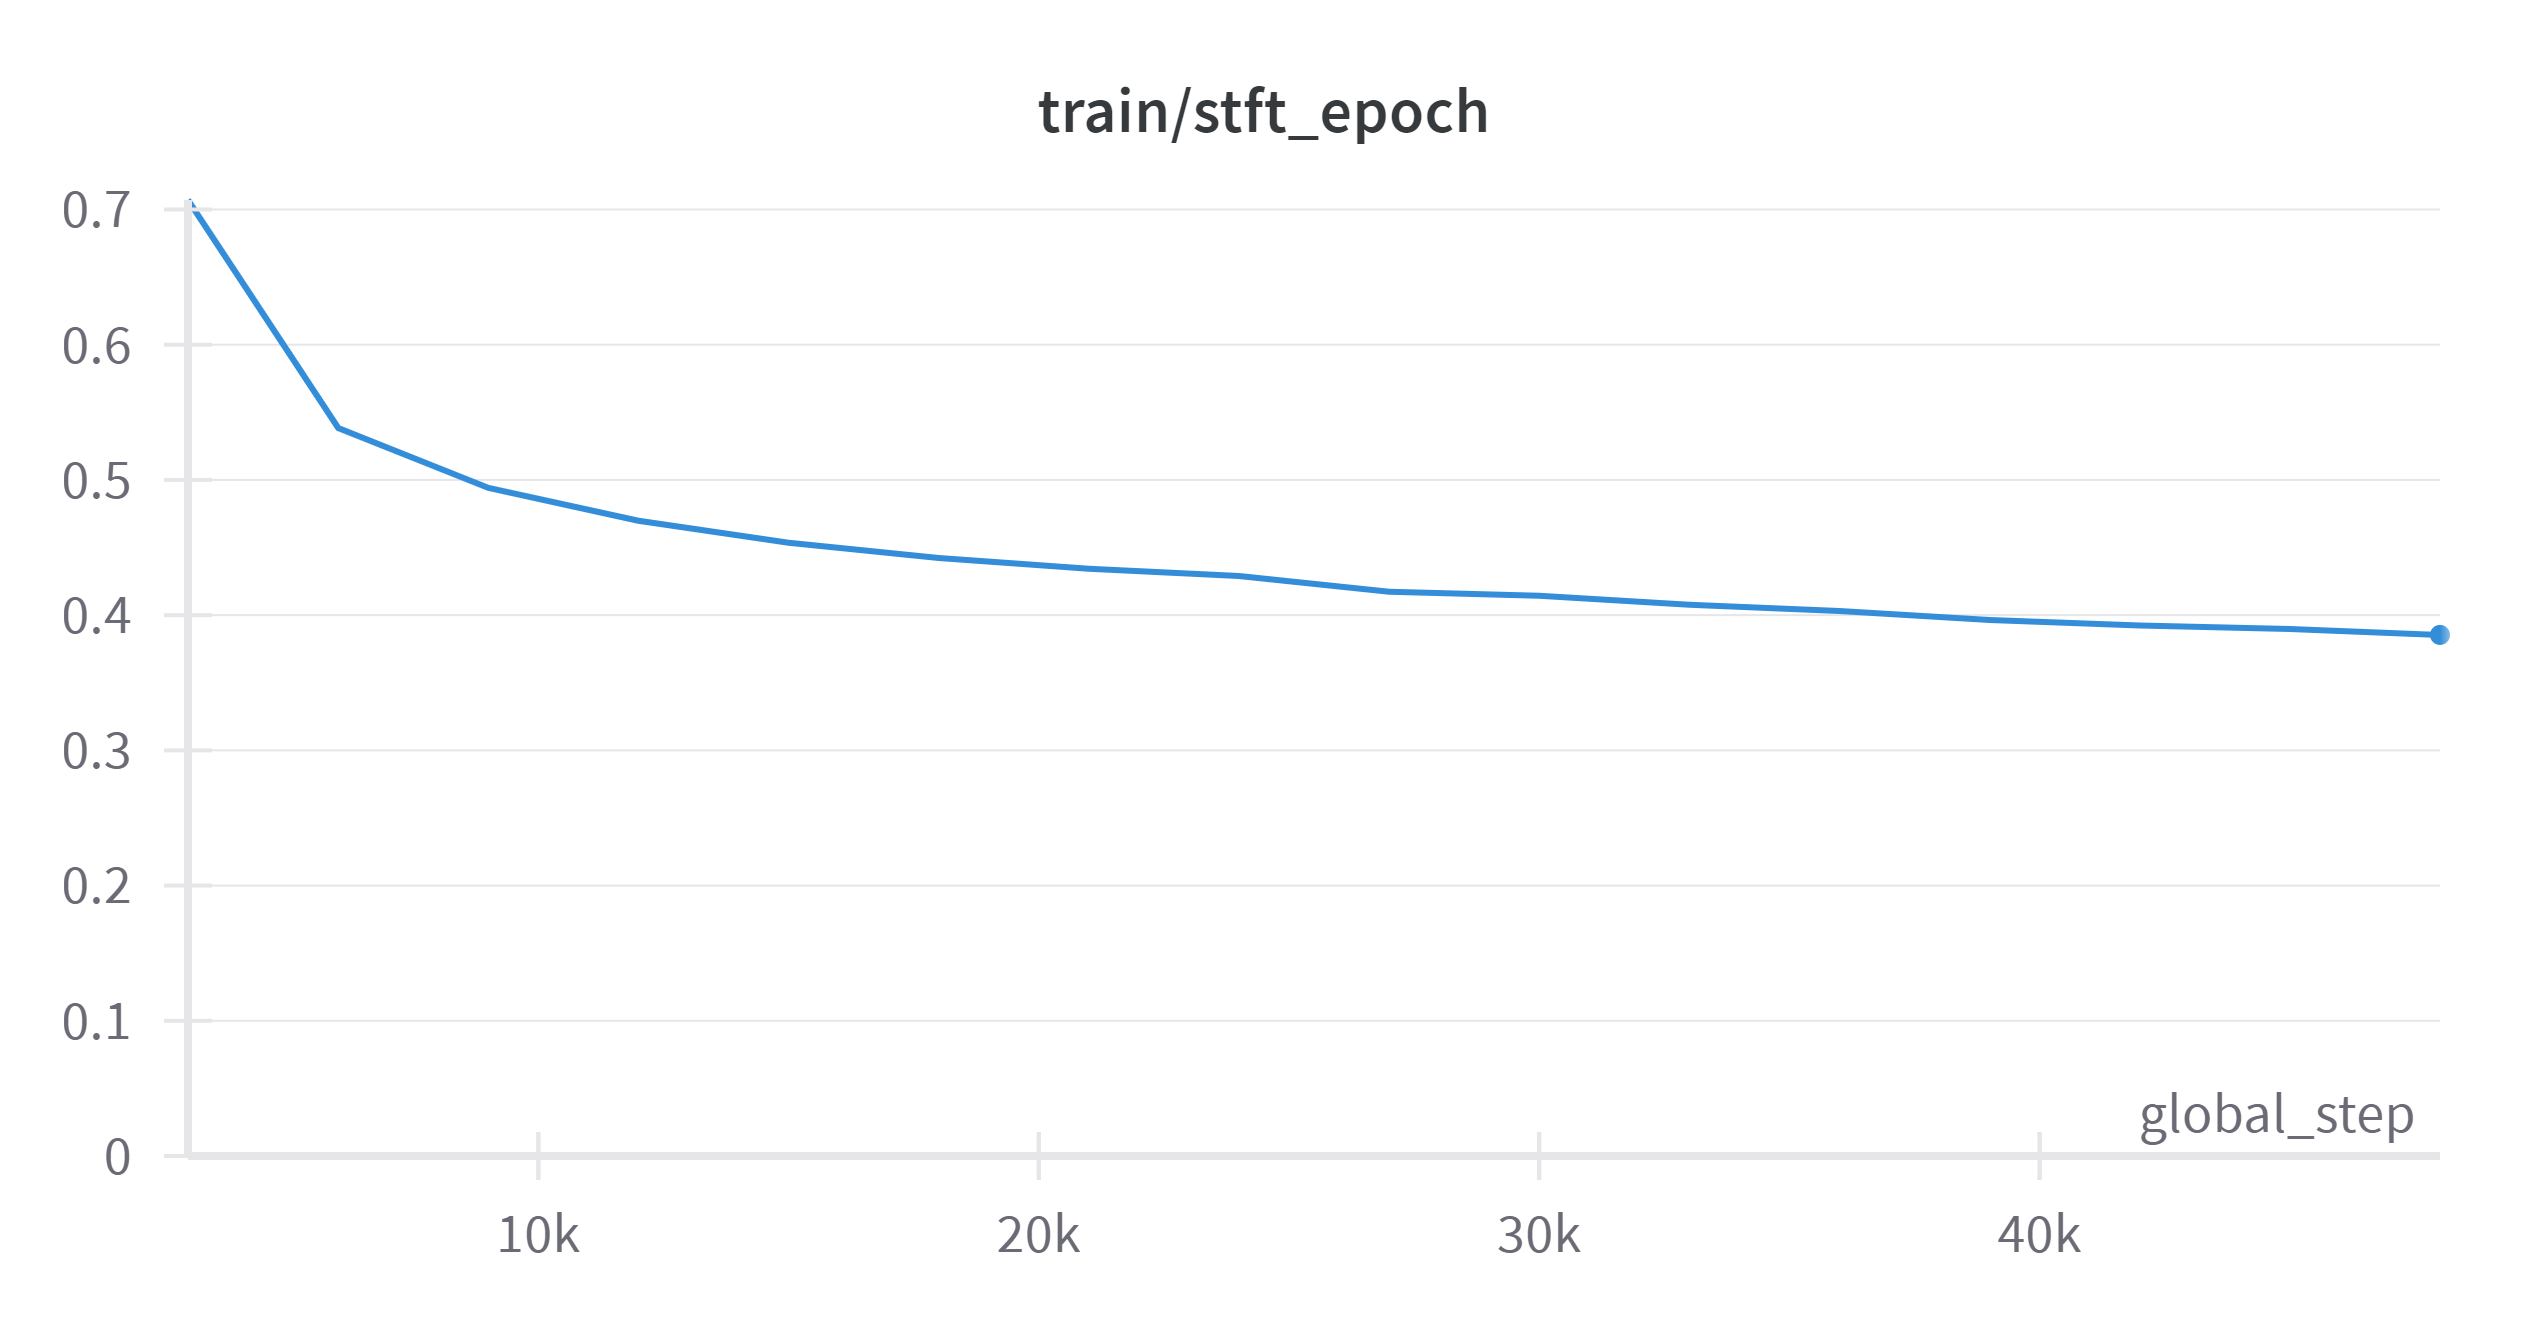
\includegraphics[width=1\linewidth]{images/experiments/cleanUnet/cleanUnet_DNS100hrs_train_stft.png}
    \caption{STFT loss reported on \\ training set.}
    \label{fig:cleanUnet_train_stft}
  \end{subfigure}
  \begin{subfigure}{.3\textwidth}
    \centering
    % includes second image
    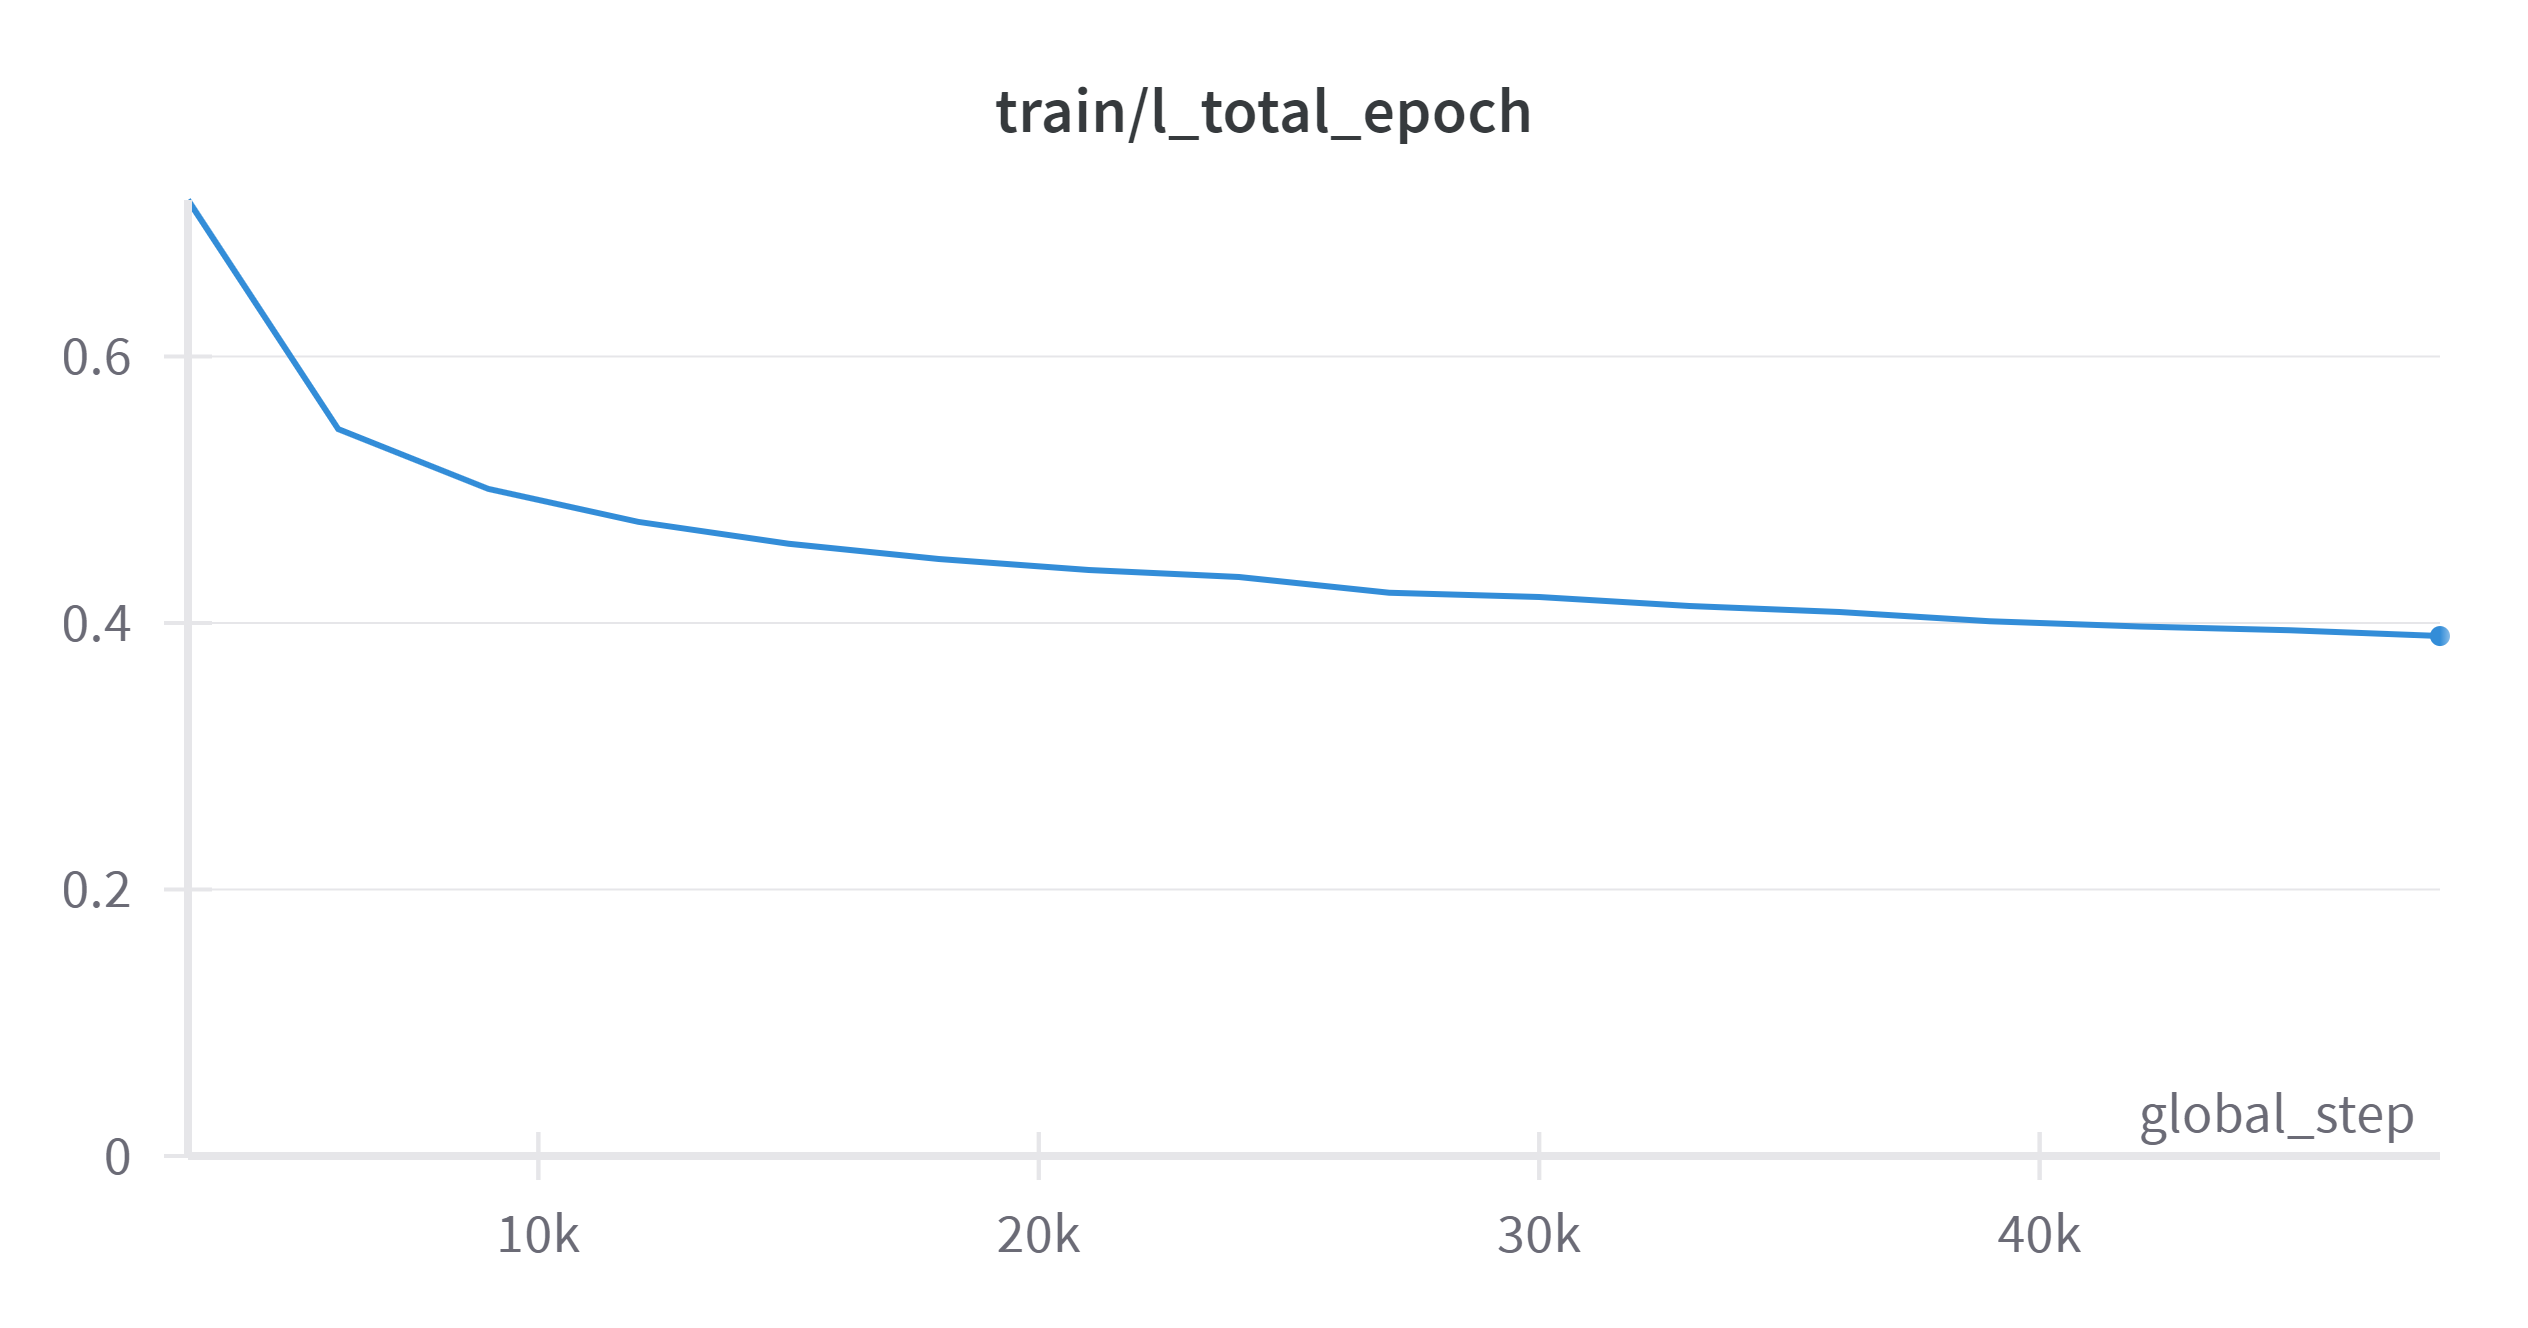
\includegraphics[width=1\linewidth]{images/experiments/cleanUnet/cleanUnet_DNS100hrs_train_total.png}
    \caption{Total loss reported on\\ training set.}
    \label{fig:cleanUnet_train_total}
  \end{subfigure}


  % \newline


  % \begin{subfigure}{.3\textwidth}
  %   \centering
  %   % include the third image
  %   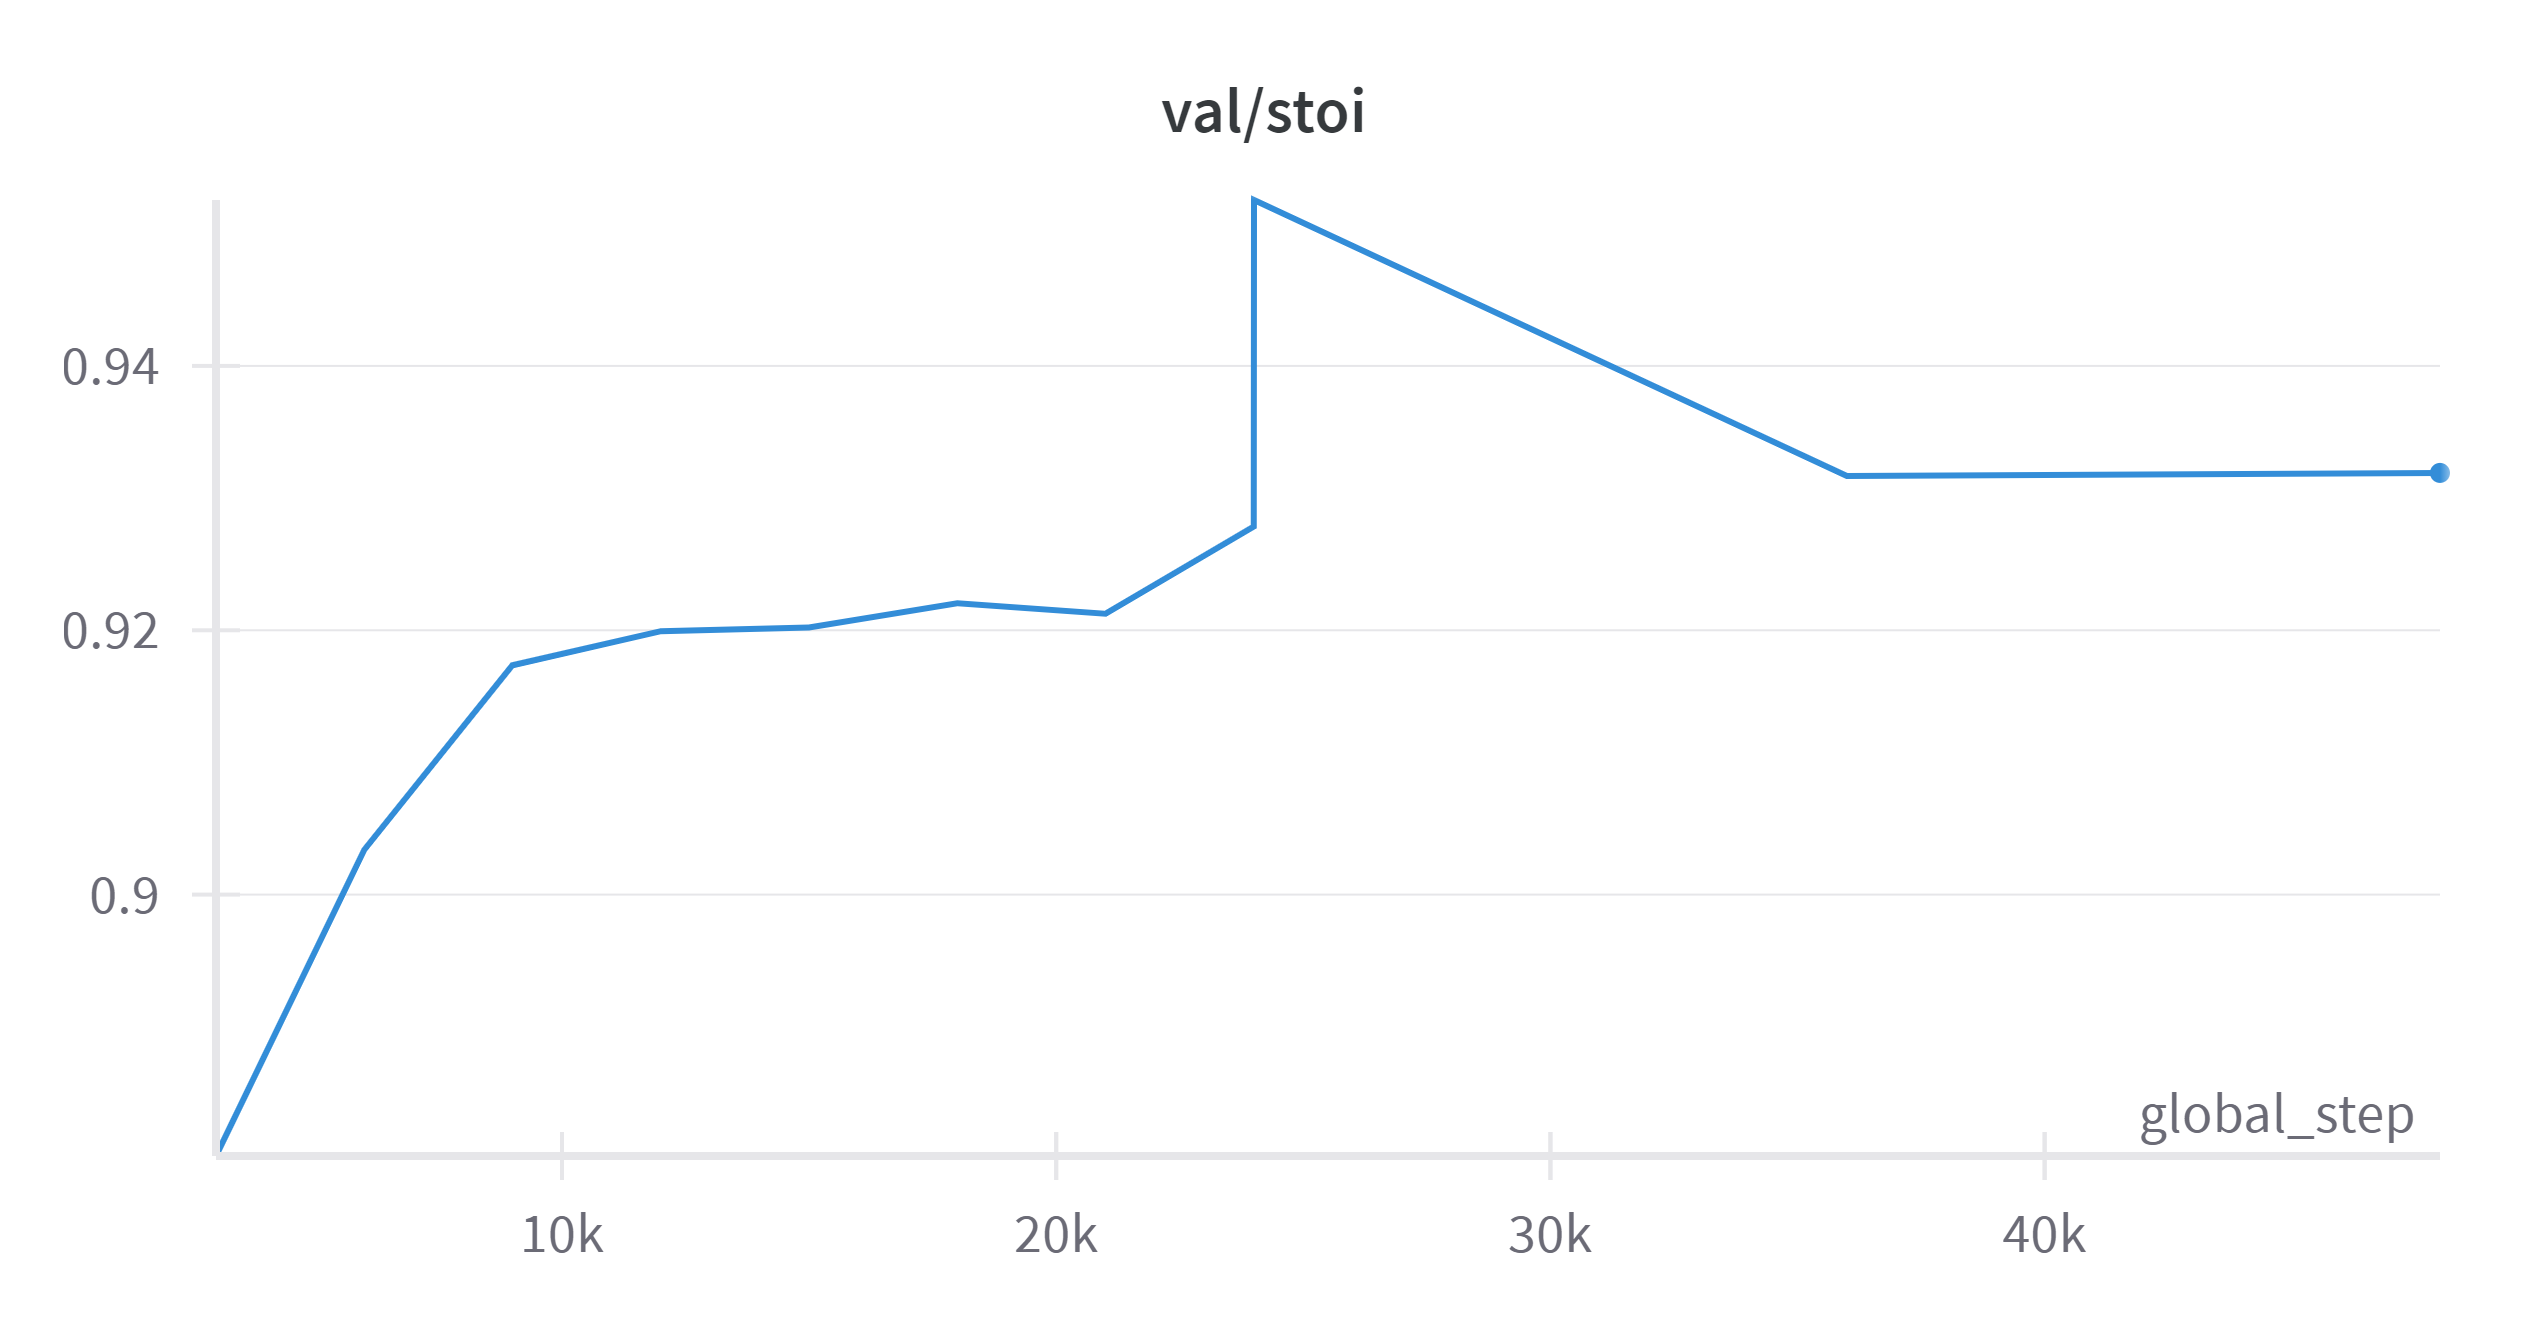
\includegraphics[width=1\linewidth]{images/experiments/cleanUnet/cleanUnet_dns100hrs_val_stoi.png}  
  %   \caption{STOI reported on\\ test set.}
  %   \label{fig:cleanUnet_val_stoi}
  % \end{subfigure}
  % \begin{subfigure}{.3\textwidth}
  %     \centering
  %     % include the fourth image
  %     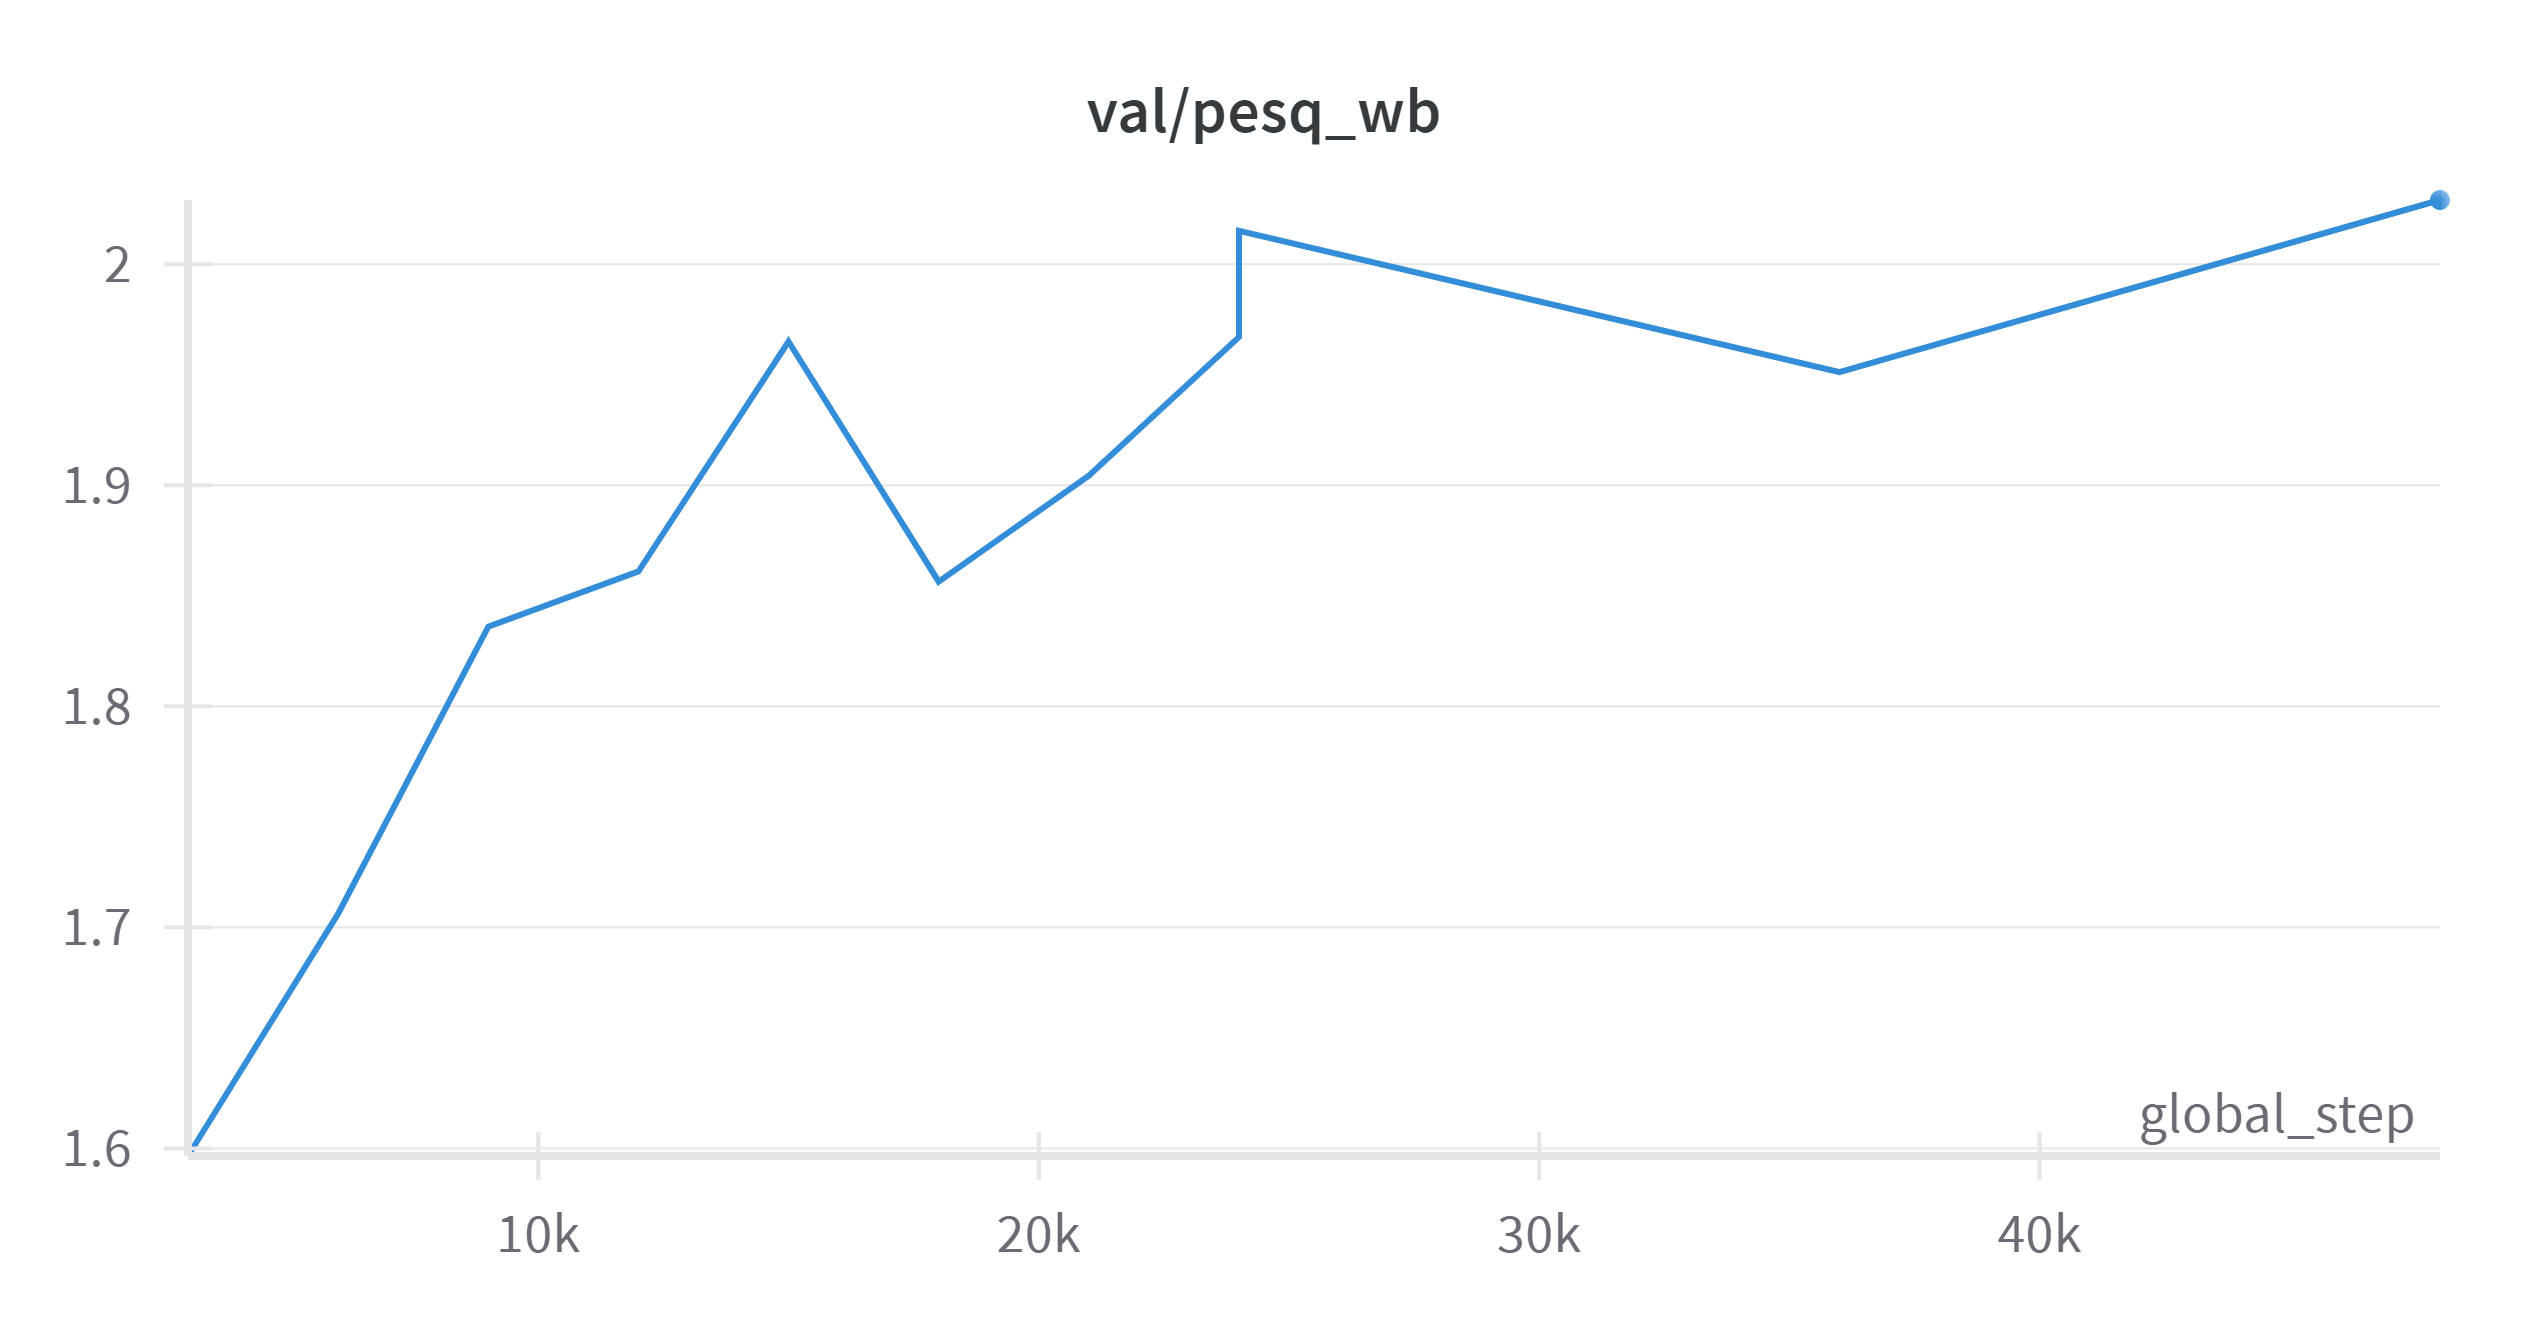
\includegraphics[width=1\linewidth]{images/experiments/cleanUnet/cleanUnet_DNS100hrs_val_pesq_wb.png}  
  %     \centering\caption{PESQ-WB reported on\\ test set.}
  %     \label{fig:cleanUnet_val_pesq_wb}
  % \end{subfigure}
  % \begin{subfigure}{.3\textwidth}
  %   \centering
  %   % include the fourth image
  %   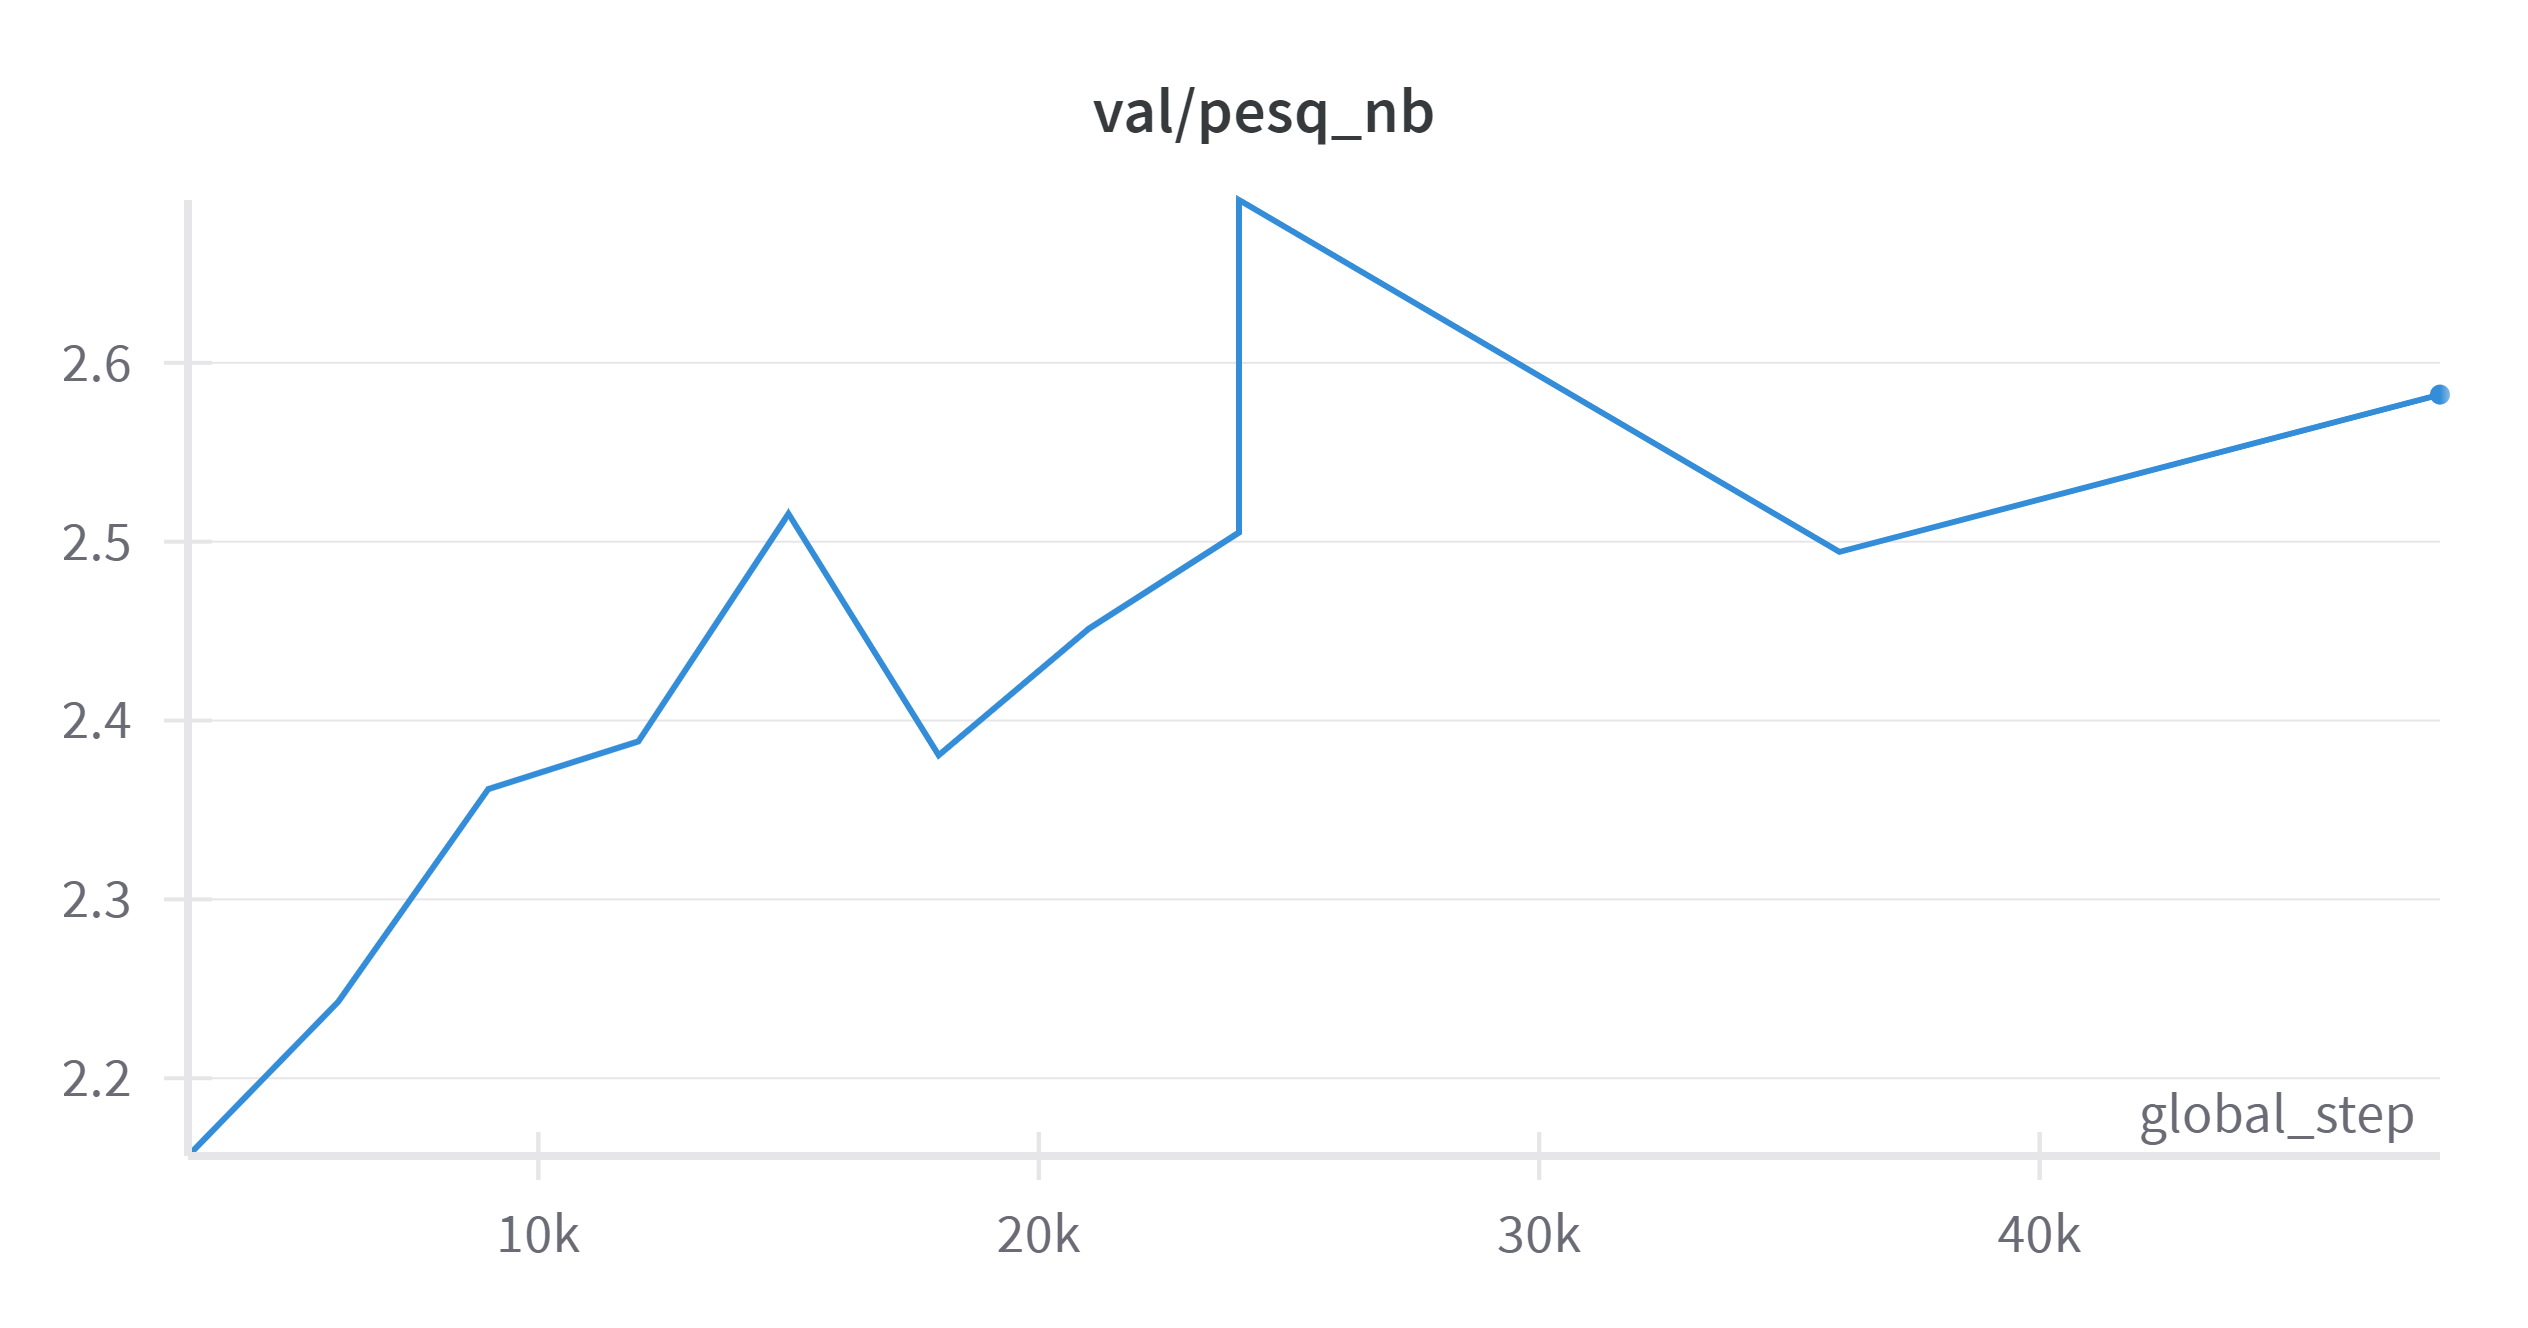
\includegraphics[width=1\linewidth]{images/experiments/cleanUnet/cleanUnet_DNS100hrs_val_pesq_nb.png}  
  %   \caption{PESQ-NB reported on\\ test set.}
  %   \label{fig:cleanUnet_val_pesq_nb}
  % \end{subfigure}
  \caption{Training logs for CleanUNet model.}
  \label{fig:cleanunet-training}
\end{figure}

\begin{table}[h]
  \centering
  \begin{tabular}{c|c|c}
    \hline
    Metric  & Reported & Reproduced \\
    \hline

    STOI    & 0.977    & 0.9319     \\
    % \hline
    PESQ-WB & 3.146    & 2.029      \\
    % \hline
    PESQ-NB & 3.551    & 2.582      \\
    \hline
  \end{tabular}
  \caption{Metrics on test set of DNS-2020 dataset (without reverb) for CleanUNet model.}
  \label{tab:cleanunet-test}

\end{table}